\section{Analysis}

\subsection{Reaching Equilibrium}
The system was considered to be in equilibrium after a pre-simulation of 50.000 timesteps. As can be seen in figure \ref{findeq}, 50.000 timesteps is indeed more than enough for the energies to be in equilibrium. After only a few thousand timesteps they show only a small fluctuation around a constant average value. For the MSD and Debye temperature, it is harder to say directly from the plot whether the system has reached equilibrium or not.
\begin{figure}[H]
	\centering
	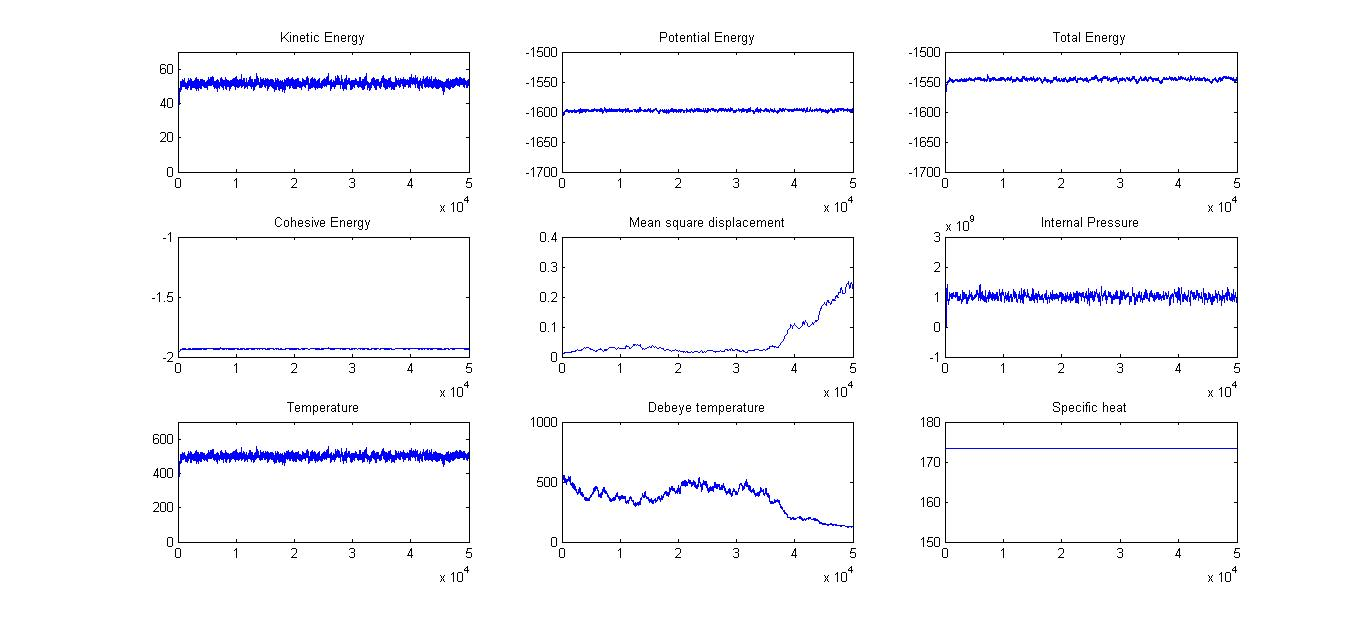
\includegraphics[width=0.7\textwidth]{findEqSurface.jpg}
	\caption{Plots of the different properties of the "pre-equilibrium" for a surface simulation.}
	\label{findeq}
\end{figure}
\subsection{Total and Cohesive Energy}
Due to the energy conservaton, the total energy should theoretically be constant for the duration of the simulation. However, there are some minor flucutations around a constant average value, at maxiumum 0.01 \% of the average value (See fig. \ref{totale} (this behavior is the same for surface as well as bulk simulations). This is thought to be due to the inevitable rounding of the values used for calculations. Since the fluctuations are very small and since the averaged value is constant, they are deemed negligible. 
The value of the total energy equals the sum of the potantial and the kinetic energy, just like it should.
\subsubsection{Cohesive energy}
The cohesive energy has an average value of 1.93 eV in the main test simulation. It is hard to find any tabulated values to compare with for that temperature, so we made a test run at T=0K also. Here, the average cohesive energy was 2.34 eV, which is not the same as, but within a reasonable range from, the tabulated value wich was found to be 2.95 eV \cite{kittel}.

\subsection{Kinetic Energy and Temperature}
The kinetic energy and the temperature are strictly connected to each other. The Andersen thermostat keeps the temperature close to its' starting value for the whole simulation.

\subsection{Potential Energy}
After reaching equilibrium, the potential energy fluctuation is less than 0.1\% of the averaged value. The fluctuations are directly related to the fluctuations of the kinetic energy, and together they sum up to the total energy.

\subsection{MSD and Diffusion Coefficient}
The MSD shows how much the atoms have moved in average from their original positions. This divided by six times the-total-time results in the diffusion coefficient which can be used to see that equilibrium is reached. The plot in figure \ref{fig:Diffusion_coeff} shows how the diffusion coefficient drops over time, for a simulation of 50,000 timesteps from the start. It can further be noticed that the diffusion coefficient seem to stabilize at the end of the run. 
\begin{figure}[ht]
	\centering
	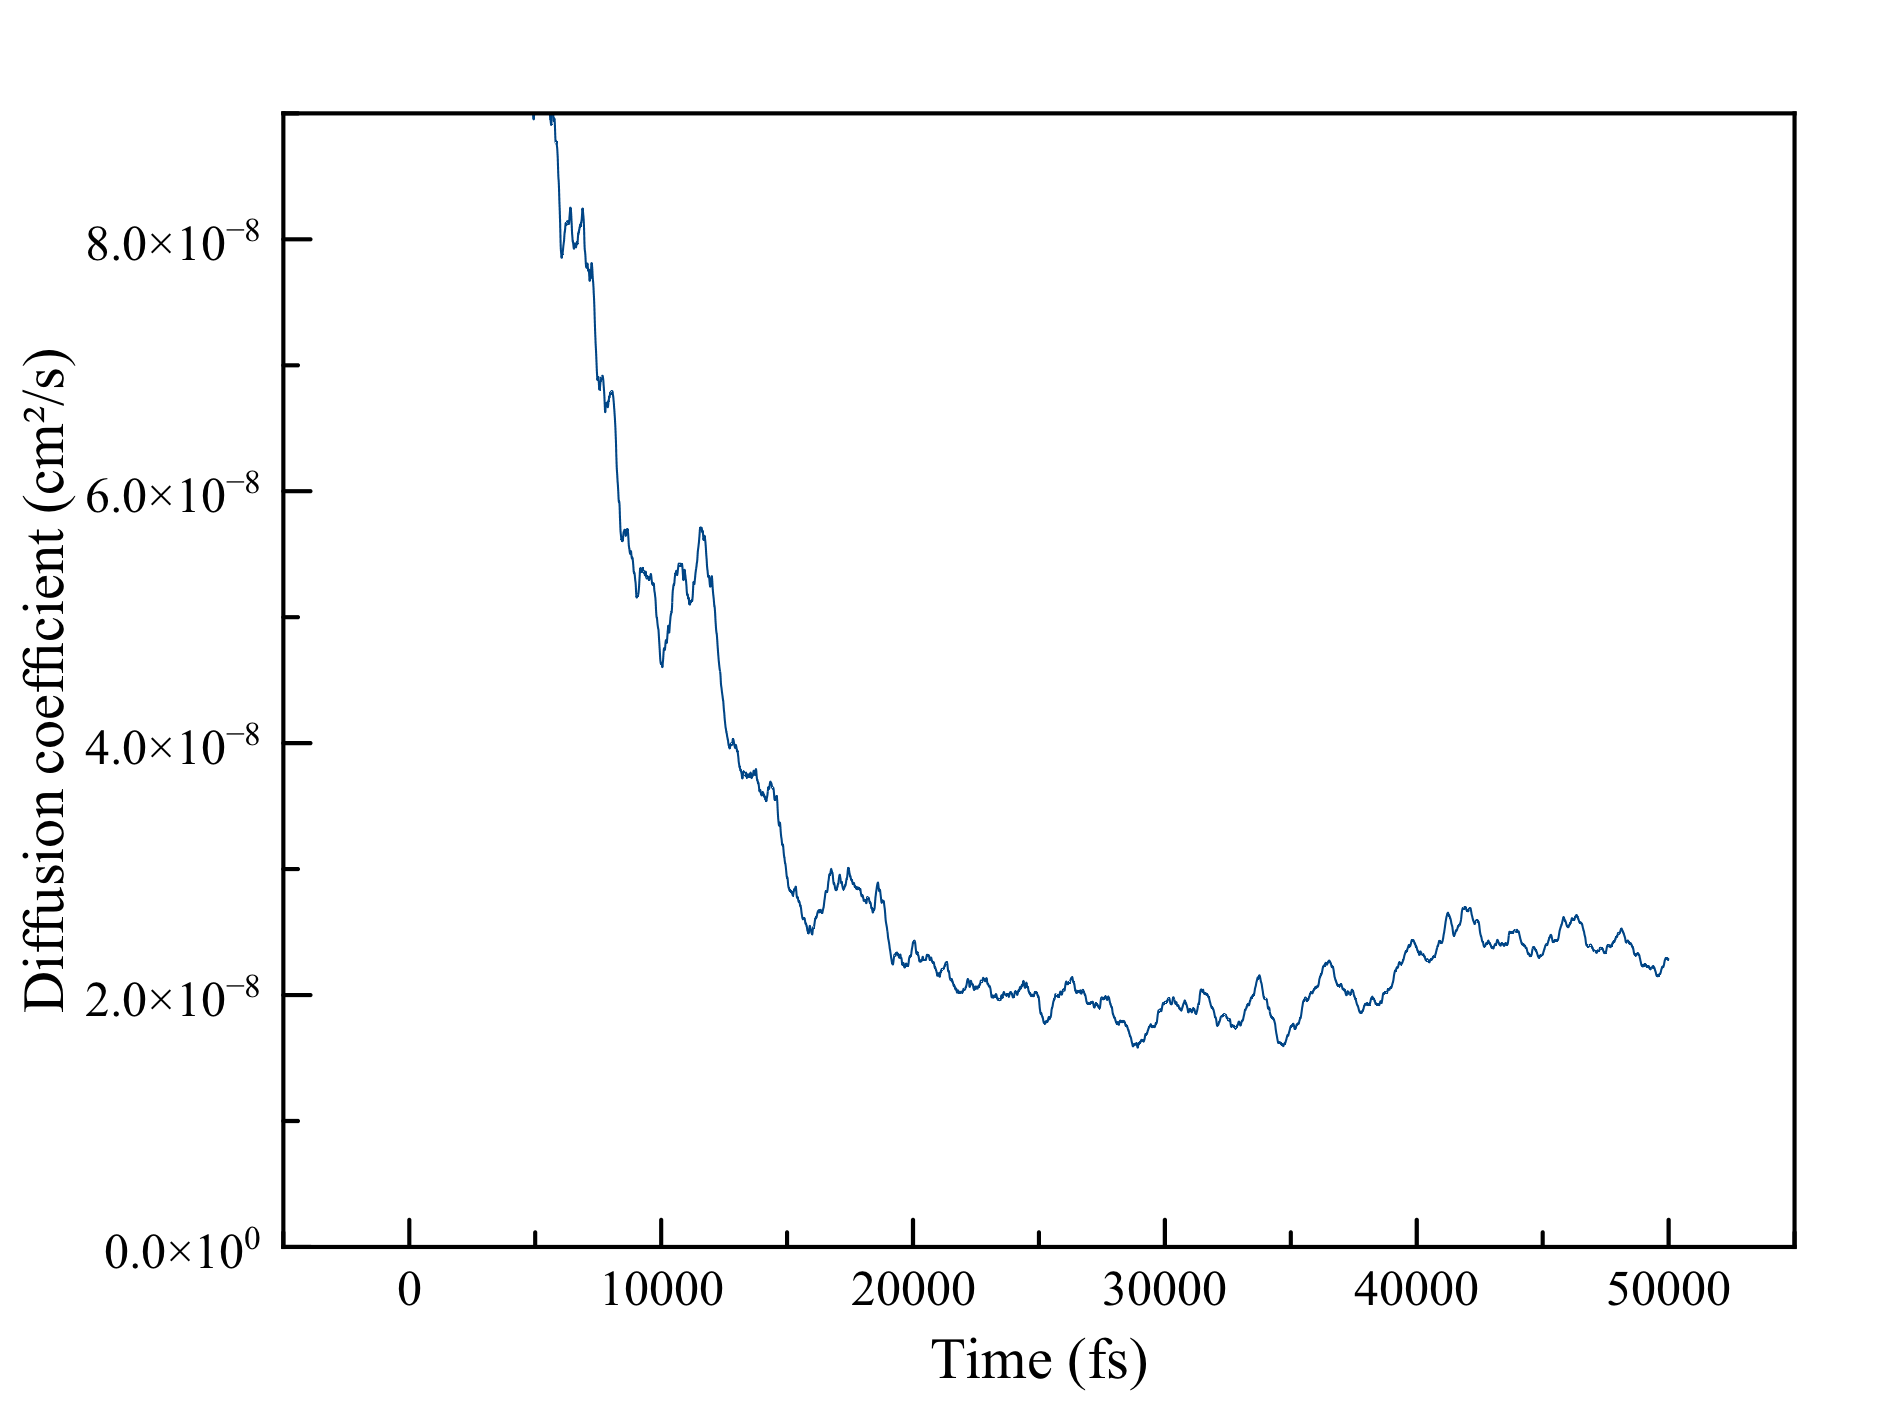
\includegraphics[width=0.5\textwidth]{Diffusion_coeff.png}
	\caption{Diffusion coefficient over time for a simulation starting at non-equilibrium}
	\label{fig:Diffusion_coeff}
\end{figure}
Furthermore, it can be seen in figure \ref{fig:diffusion_coeff_surface}, which is a plot of the diffusion coefficient for a surface simulation started at equilibrium (50,000 timesteps), that the diffusion coefficient has indeed stabilized.
\begin{figure}[ht]
	\centering
	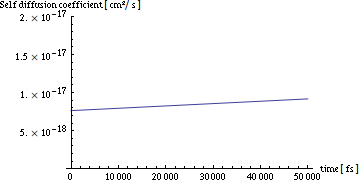
\includegraphics[width=0.7\textwidth]{diffusion_coeff_surface.png}
	\caption{Diffusion coefficient over time for a surface simulation started at equilibrium}
	\label{fig:diffusion_coeff_surface}
\end{figure}

\subsection{Debye Temperature}
The Debye temperature is inveresely proportional to the MSD and proportional to the temperature, which are used for the calculation in this program.
The value stabilizes around 250 K (see figure \ref{fig:debyetemp}) which is in good agreement with the tabulated value (215K) \cite{bib:DebyeSilver}.
\begin{figure}[ht]
	\centering
	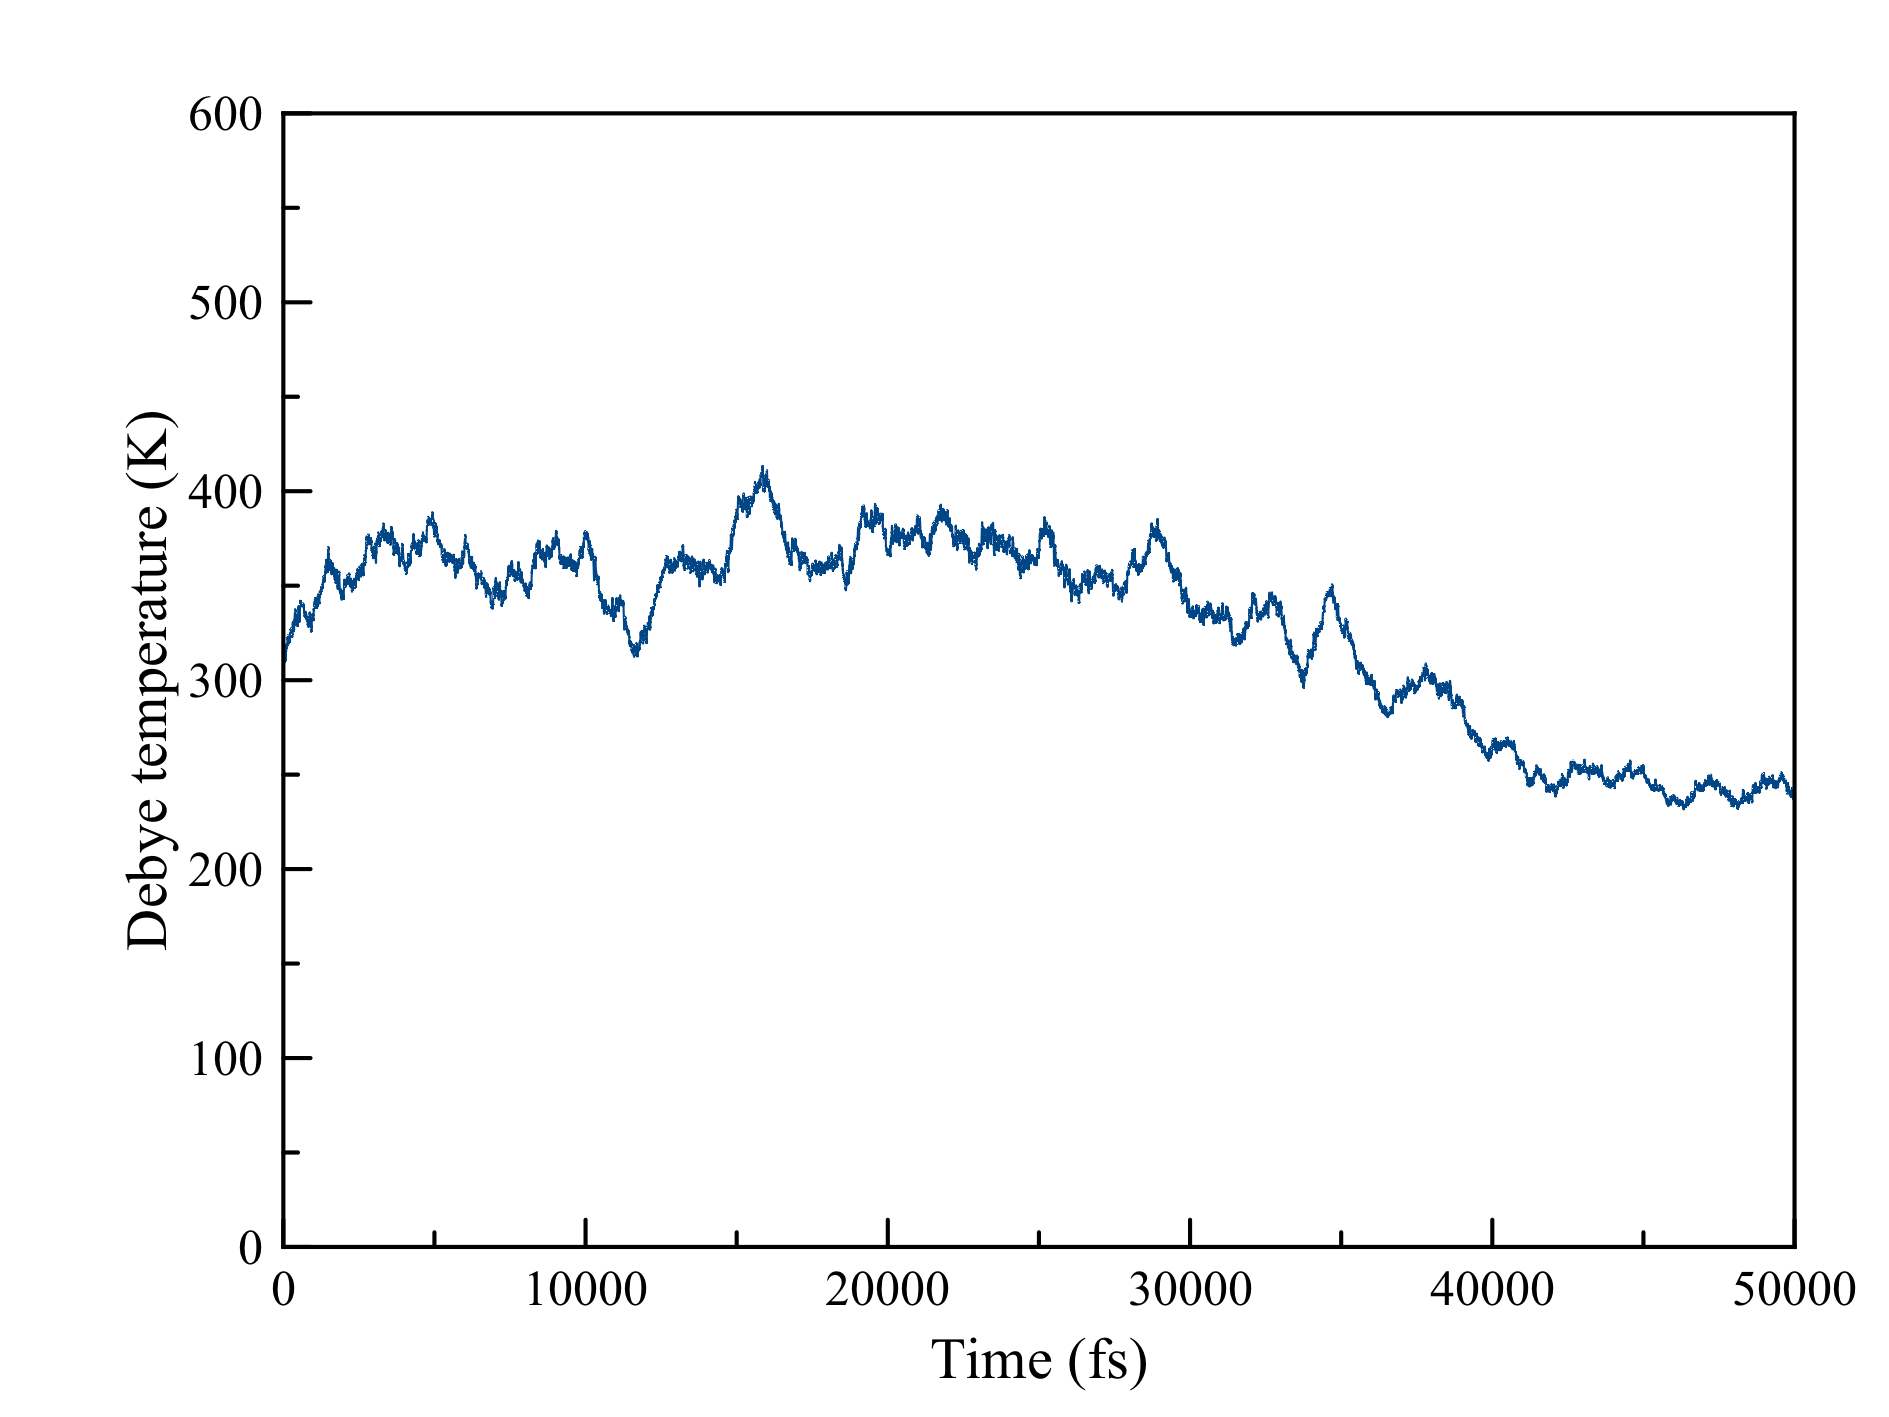
\includegraphics[width=0.7\textwidth]{debyetemp.png}
	\caption{Debye temperature for a bulk}
	\label{fig:debyetemp}
\end{figure}
For the surface simulations, the Debye temperature is a bit lower than for the bulk simulations as seen in figure \ref{fig:debye_surface}.
\begin{figure}[ht]
	\centering
	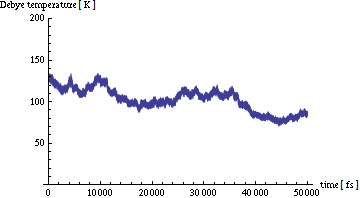
\includegraphics[width=0.7\textwidth]{debye_surface.png}
	\caption{Debye temperature for a surface}
	\label{fig:debye_surface}
\end{figure}

